\documentclass{article}

\usepackage{longtable,fancyhdr}
\usepackage{amsmath}
\usepackage{amsfonts}
\usepackage{amssymb}
\usepackage{color}

\setlength{\topmargin}{-0.5cm}
\setlength{\textheight}{23cm}
\setlength{\textwidth}{16cm}
\setlength{\oddsidemargin}{0.5cm}
\renewcommand{\baselinestretch}{1.1}
\renewcommand{\topfraction}{0.99}
\renewcommand{\bottomfraction}{0.99}

\def\Y{{\rm Y}}
%\def\var{{\rm var}}
\def\var{\hbox{var}}
\def\npde{{\rm npde}}
\def\pde{{\rm pde}}
\def\npd{{\rm npd}}
\def\pd{{\rm pd}}
\def\vec{{\rm vec}}
\def\ypred{{\rm ypred}}
\def\R{{\sf R}}
\def\true{{\sf TRUE}}
\def\false{{\sf FALSE}}

\title{Tuning graphs in the npde library}
\author{Emmanuelle Comets}
\date{\today}

%\definecolor{violet}{rgb}{0.25,0.1,0.75}
%\definecolor{mycol}{rgb}{0.5,0.1,0.6}

\usepackage{Sweave}
\begin{document}
\Sconcordance{concordance:demoGraphs.tex:demoGraphs.Rnw:%
1 63 1 1 9 36 1 1 38 9 0 1 23 1 3 6 1 1 2 3 0 1 5 21 %
0 1 2 2 0 1 1 2 0 1 12 43 0 1 2 4 1 1 2 4 0 1 2 2 1 2 %
2 12 1 2 2 37 1 1 2 5 0 1 2 7 1 1 2 5 0 1 2 104 1 1 2 %
23 0 1 11 2 1 1 2 5 0 1 2 7 1 1 2 6 0 1 3}


\pagestyle{fancy}
\renewcommand{\headrulewidth}{0pt}
\renewcommand{\footrulewidth}{1pt}
%\renewcommand{\footrulewidth}{0pt}
\lhead{}
\chead{}
\rhead{}
\lfoot{\itshape E. Comets, \today}
\cfoot{Beautiful graphs with npde 3.0}
\rfoot{\thepage}

% From R. Ihaka (customising Sweave output)
% Indenting
\DefineVerbatimEnvironment{Sinput}{Verbatim}{xleftmargin=2em,fontshape=sl,fontfamily=tt}
\DefineVerbatimEnvironment{Soutput}{Verbatim}{xleftmargin=2em,fontshape=sl,fontfamily=tt}
\DefineVerbatimEnvironment{Scode}{Verbatim}{xleftmargin=2em,fontshape=sl,fontfamily=tt}
\fvset{listparameters={\setlength{\topsep}{-1pt}}}
\renewenvironment{Schunk}{\vspace{\topsep}}{\vspace{\topsep}}

\parindent 18pt
$\phantom{minime}$

\vskip 3cm
\begin{center}
{\setlength{\baselineskip}{2\baselineskip}
{\Large \bfseries Beautiful graphs with npde 3.0}

{\Large \bfseries September 2020}

\bigskip 

{\Large \itshape \bfseries Emmanuelle Comets, Romain Leroux}

\bigskip 

\bigskip 

{\large \itshape \bfseries Contributors to npde: Karl Brendel, Marc Cerou, Romain Leroux, Thi Huyen Tram Nguyen, France Mentr\'e}

\bigskip
{\it
INSERM, IAME UMR 1137, Paris, France

Universit\'e de Paris, Paris, France.
}
\par}
\end{center}

\vskip 8cm
\begin{center}
{\large \bfseries npde website: www.npde.biostat.fr}
\end{center}

\newpage
% Loading libraries:

\section{Running npde }

Describe:
- viral load data example
  - 20\% 

\begin{Schunk}
\begin{Soutput}
Viral load data with 20% censored data
\end{Soutput}
\begin{Soutput}
[1] "computenpde.loq<-function(npdeObject) {"
---------------------------------------------
Distribution of npde :
      nb of obs: 300 
           mean= -0.03127   (SE= 0.053 )
       variance= 0.8358   (SE= 0.068 )
       skewness= 0.04592 
       kurtosis= -0.3856 
---------------------------------------------

Statistical tests
  t-test                     : 0.554
  Fisher variance test       : 0.0355 *
  SW test of normality       : 0.499
Global adjusted p-value      : 0.107
---
Signif. codes: '***' 0.001 '**' 0.01 '*' 0.05 '.' 0.1 
---------------------------------------------
\end{Soutput}
\begin{Soutput}
Warfarin PK data
\end{Soutput}
\begin{Soutput}
      npde for the model without covariates
\end{Soutput}
\begin{Soutput}
---------------------------------------------
Distribution of npde :
      nb of obs: 247 
           mean= 0.03419   (SE= 0.06 )
       variance= 0.8753   (SE= 0.079 )
       skewness= -0.1149 
       kurtosis= -0.0497 
---------------------------------------------

Statistical tests
  t-test                     : 0.566
  Fisher variance test       : 0.157
  SW test of normality       : 0.371
Global adjusted p-value      : 0.471
---
Signif. codes: '***' 0.001 '**' 0.01 '*' 0.05 '.' 0.1 
---------------------------------------------
      npde for the model with covariates
---------------------------------------------
Distribution of npde :
      nb of obs: 247 
           mean= 0.02928   (SE= 0.059 )
       variance= 0.8549   (SE= 0.077 )
       skewness= -0.07211 
       kurtosis= -0.4172 
---------------------------------------------

Statistical tests
  t-test                     : 0.619
  Fisher variance test       : 0.096 .
  SW test of normality       : 0.368
Global adjusted p-value      : 0.288
---
Signif. codes: '***' 0.001 '**' 0.01 '*' 0.05 '.' 0.1 
---------------------------------------------
\end{Soutput}
\end{Schunk}

The {\sf npde} package has built-in diagnostic plots which can be accessed for an object {\sf y} returned by \verb+autonpde()+ (or \verb+npde()+ for the interactive execution) by the usual R command \verb+plot()+:
\begin{verbatim}
plot(y)
\end{verbatim}
\begin{Schunk}
\begin{Sinput}
> plot(yvir20)
\end{Sinput}
\end{Schunk}
produces the plot shown in figure~\ref{fig:defaultVL20}.  
\begin{figure}[!h]
\begin{center}
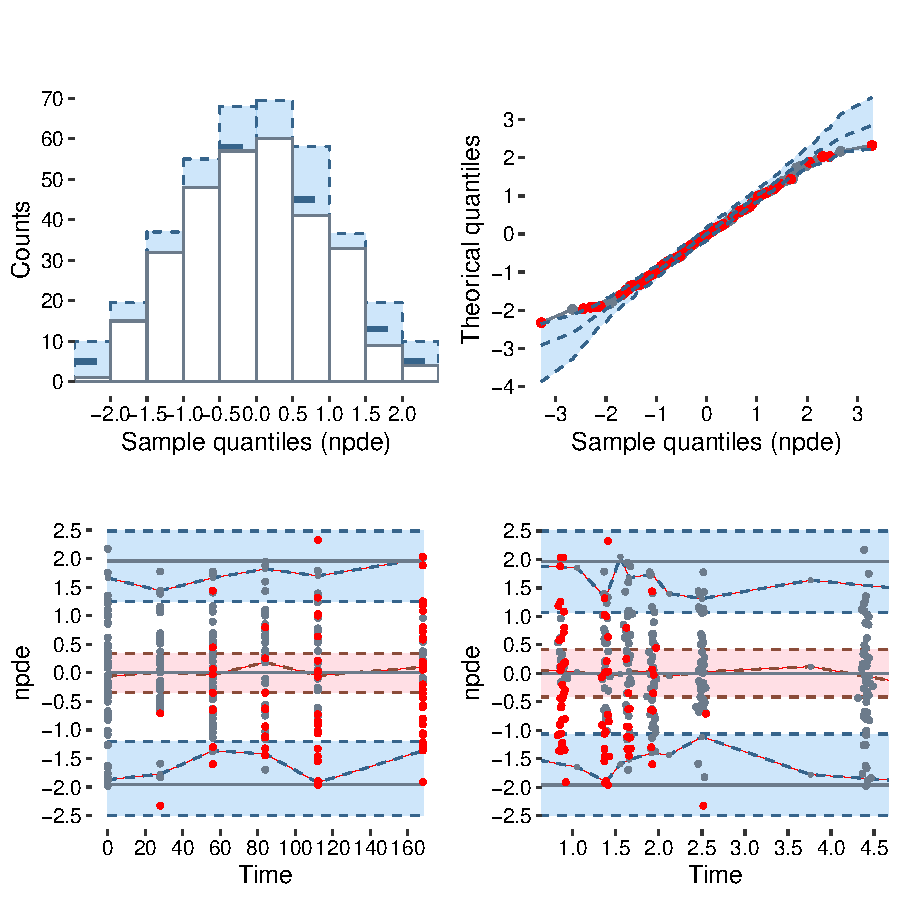
\includegraphics{demoGraphs-defplotsVir20}
\end{center}
\par \kern -0.5cm
\caption{Default plots for the viral load data.} \label{fig:defaultVL20}
\end{figure}

{\bfseries Eco TODO problems with the viral load data plots:}
\begin{itemize}
\item not the same result when I execute interactively the viral load data (the p-value is NS interactively, but sometimes comes out significant)
\item check the nubmer of simulations, maybe not enough ?
\end{itemize}

\begin{figure}[!h]
\begin{center}
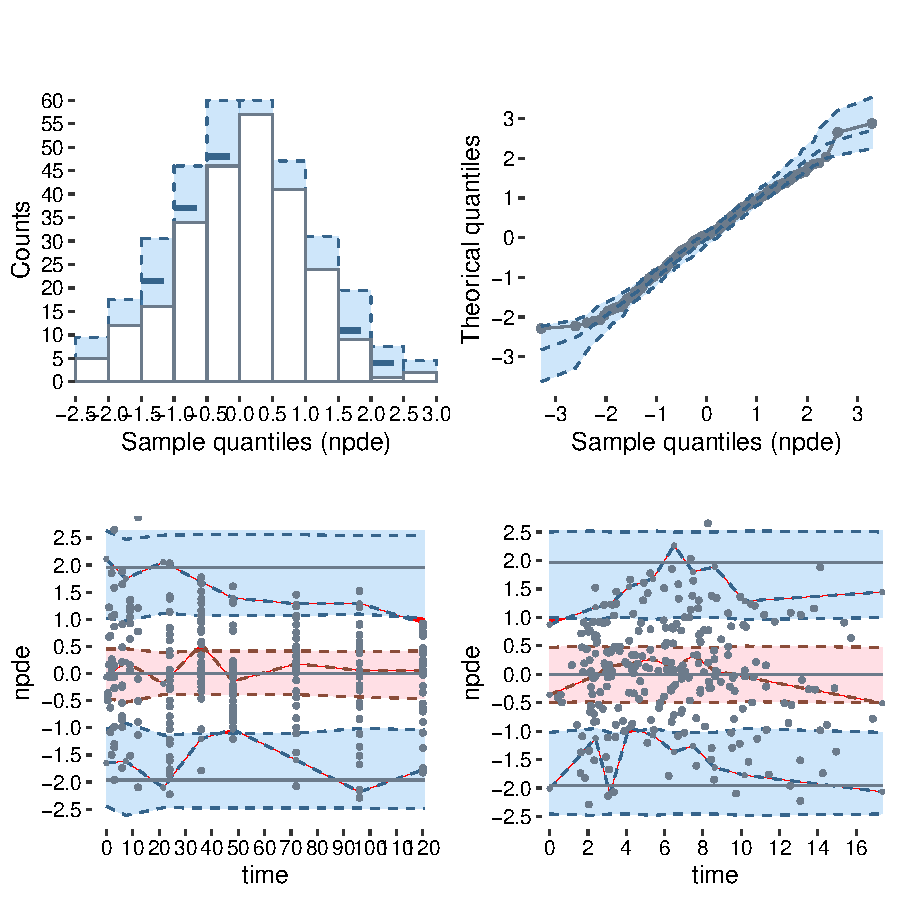
\includegraphics{demoGraphs-defplotsWarfBase}
\end{center}
\par \kern -0.5cm
\caption{Default plots for the warfarin PK data, assuming a model without covariates.} \label{fig:defWbase}
\end{figure}

\clearpage
\newpage
\section{Graphical options}

\subsection{Types of plots} \label{sec:plotTypes}

\hskip 18pt Each of the default diagnostic plots, as well as a number of additional plots not shown by default, can also be produced on its own, using the argument \verb+plot.type="type"+. Table~\ref{tab:plottypes} lists the plots that can be created in this way. Apart from VPC and the plot of the probability of an observation being under the LOQ, all plots can be obtained for \npde, \npd or \pd (this is controlled by the \verb+which=""+ argument, defaulting to \verb+which="npde"+).

\begin{table}[!h]
%\noindent{\bfseries Table II:} {\itshape Types of plots available.}
%\label{tab:plot.types}
\begin{center}
\begin{tabular} {| r p{10cm} |}
\hline {\bf Plot type} & {\bf Description} \\
\hline
data & Plots the observed data in the dataset \\
hist & Histogram of the \npde \\
qqplot & QQ-plot of the \npde versus its theoretical distribution  \\
ecdf & Empirical distribution function of the \npde\\
x.scatter & Scatterplot of the \npde~versus the predictor X \\
pred.scatter & Scatterplot of the \npde~versus the population predicted values \\
cov.scatter & Scatterplot of the \npde~versus covariates \\
vpc & Plots a Visual Predictive Check (VPC) \\
loq & Plots the probability for an observation to be BQL, versus the predictor X \\
\hline
\end{tabular}
\end{center}
\caption{Plot types available in the {\sf npde} library. QQ-plots, histograms, cumulative cdf, and scatter plots can be produced for \npde, \pd~or \npd.} \caption{tab:plottypes}
\end{table}

To produce only the QQ-plot as a standalone graph, we request a "qqplot":
\begin{figure}[!h]
\begin{center}
\begin{Schunk}
\begin{Sinput}
> plot(yvir20, plot.type="qqplot")
\end{Sinput}
\end{Schunk}
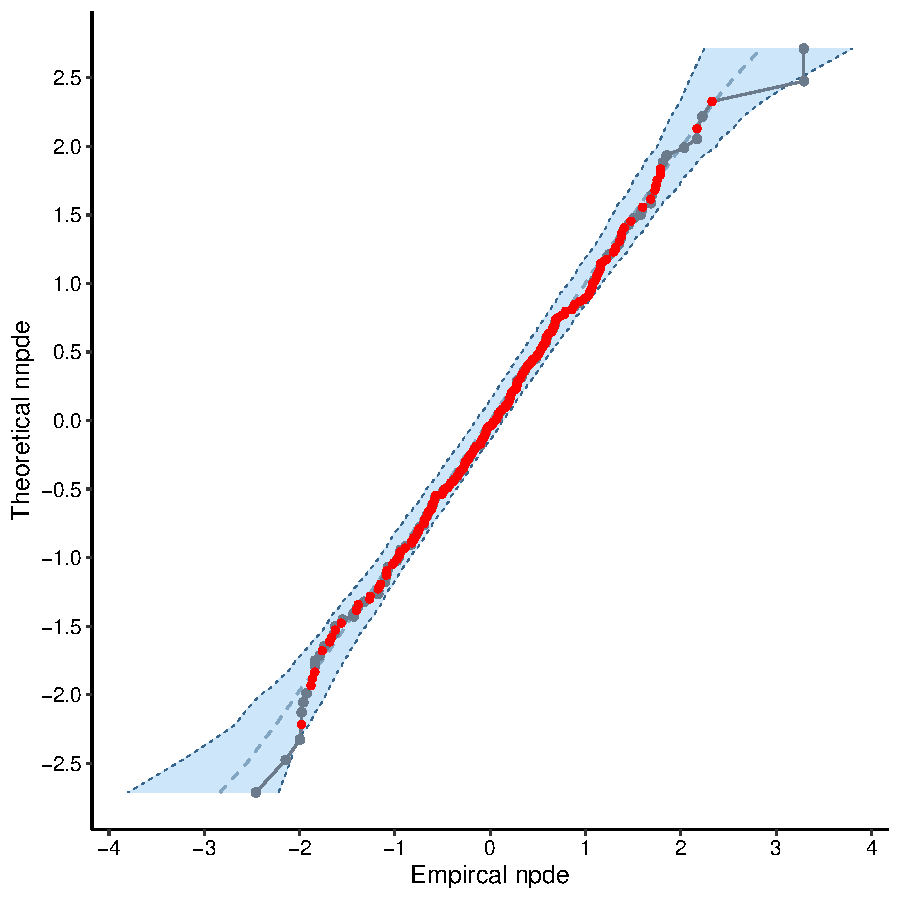
\includegraphics{demoGraphs-qqplotVL20}
\end{center}
\par \kern -0.5cm
\caption{QQ-plot for the viral load data.} \label{fig:qqplotVL20}
\end{figure}

The plots can also be produced by the other metrics computed by \verb+npde()+, for instance we might want to consider the histogram of \pd with the following command:
\begin{figure}[!h]
\begin{center}
\begin{Schunk}
\begin{Sinput}
> plot(yvir20, plot.type="hist",which="pd")
\end{Sinput}
\end{Schunk}
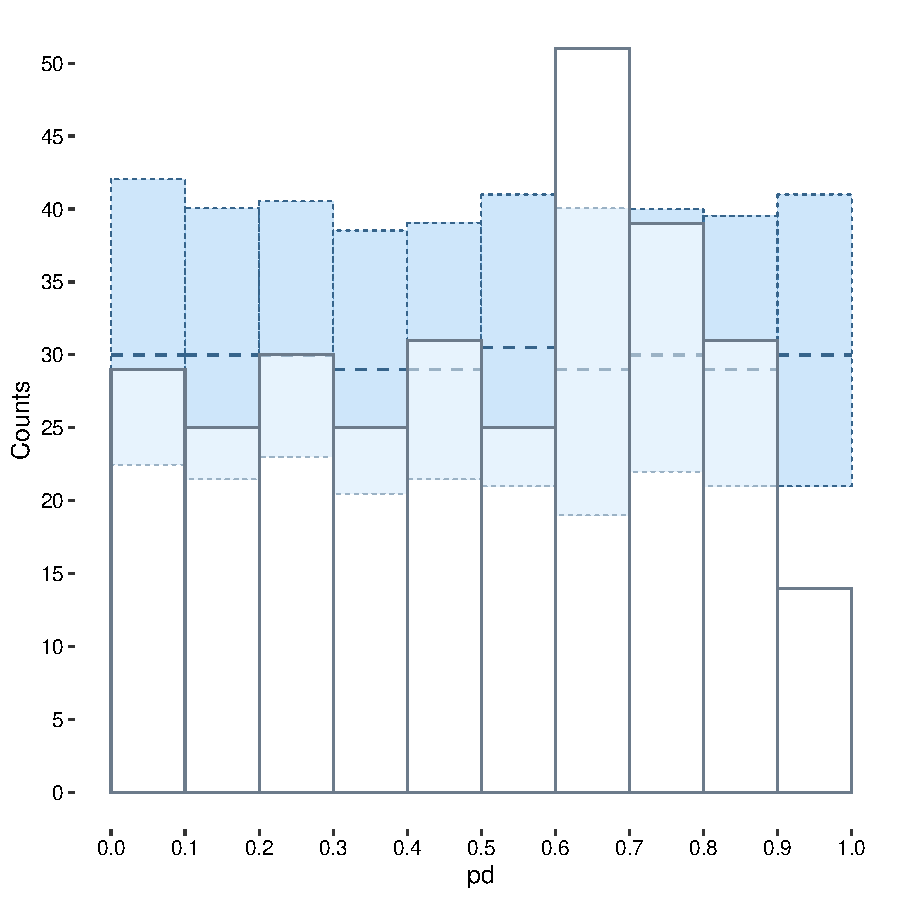
\includegraphics{demoGraphs-histVL20pd}
\end{center}
\par \kern -0.5cm
\caption{Histogram for the pd, computed in the viral load data example.} \label{fig:histVL20pd}
\end{figure}

\clearpage
\newpage
\subsection{Changing graphical parameters}

\hskip 18pt TODO: show different features in group, eg colours/symbols, titles/axes, boxes/grids

Decide on following options: verbose 

\begin{table}[!h] 
\begin{center}
\begin{tabular}{| r p{8cm} c|}
\hline
\textbf{\textcolor{black}{Argument}} & \centering{\textbf{\textcolor{black}{Description }}} & \textbf{\textcolor{black}{Default value}} \\
\hline
{\ttfamily verbose} & Output is produced for some plots (most notably when binning is used, this prints out the boundaries of the binning intervals) if TRUE & FALSE \\
{\ttfamily main} & Title & depends on plot \\
{\ttfamily sub } & Subtitle & empty \\
{\ttfamily size.main } & Size of the main title & 14 \\
{\ttfamily size.sub  } & Size of the title for covariate & 12 \\

{\ttfamily xlab} & Label for the X-axis & depends on plot \\
{\ttfamily ylab} & Label for the Y-axis & depends on plot \\
{\ttfamily size.xlab} & Size of the label for the X-axis & 12 \\
{\ttfamily size.ylab} & Size of the label for the Y-axis & 12 \\
{\ttfamily breaks.x} & Number of tick marks on the X-axis & 10 \\
{\ttfamily breaks.y} & Number of tick marks on the Y-axis & 10 \\
{\ttfamily size.x.text} & Size of tick marks and tick labels on the X-axis & 10 \\
{\ttfamily size.y.text} & Size of tick marks and tick labels on the Y-axis & 10 \\

{\ttfamily xlim} & Range of values on the X-axis & empty, adjusts to the data \\
{\ttfamily ylim} & Range of values on the Y-axis & empty, adjusts to the data \\

{\ttfamily xaxt} & A character whether to plot the X axis. Specifying "n" suppresses plotting of the axis & "y"  \\
{\ttfamily yaxt} & A character whether to plot the Y axis. Specifying "n" suppresses plotting of the axis & "y" \\

{\ttfamily xlog} & Scale for the X-axis (TRUE: logarithmic scale) & FALSE \\
{\ttfamily ylog} & Scale for the Y-axis (TRUE: logarithmic scale) & FALSE \\

{\ttfamily } & &  \\
\hline
\end{tabular} 
\end{center}
\caption{Graphical parameters that can be passed on the plot function: titles and axes.} \label{tab:graphicalOptions1}
\end{table} 


\begin{table}[!h] 
\begin{center}
\begin{tabular}{| r p{8cm} c|}
\hline
\textbf{\textcolor{black}{Argument}} & \centering{\textbf{\textcolor{black}{Description }}} & \textbf{\textcolor{black}{Default value}} \\
\hline
{\ttfamily col} & Main colour for observed data (applied to lines and symbols pertaining to observations if no other option is given to supersede this value) & "slategray4"  \\
{\ttfamily lty} & Line type for observed data & 1 \\
{\ttfamily lwd} & Line width for observed data & 0.5 \\
{\ttfamily pch} & Symbol used to plot observed data &  20 \\
{\ttfamily alpha} & Transparencyfor observed data  & 1 \\
{\ttfamily size} & Symbol size to plot observed data & 1  \\
{\ttfamily fill} & Colour used to fill area elements related to observed data (such as histogram bars) & "white  \\
{\ttfamily } & &  \\
\hline
\end{tabular} 
\end{center}
\caption{Graphical parameters that can be passed on the plot function: colours and symbols.} \label{tab:graphicalOptions2}
\end{table} 


\clearpage
\newpage

\subsection{Saving to file}

\subsubsection{Using ggsave from ggplot}

\subsubsection{Handling transparency with postscript files}

Postcript doesn't handle the transparency used in the {\sf npde} plots made with the {\sf ggplot2} library. Using {\sf ggsave()}, the prediction intervals will likely be missing from the output. A workaround is to output the files to PDF format. Another is to use the following code

{\bf TODO}

\subsection{Arranging individual plots}

\section{Covariate plots}

\subsection{Plots of {\bfseries npde} versus covariates}

\subsection{Stratified plots}

\hskip 18pt The different diagnostic plots produced in section~\ref{sec:plotTypes} can be stratified using the \verb+covsplit=TRUE+ option. By default, the plots will be stratified for each covariate separately. The plots produced depend on the nature of the covariate, following~\cite{Brendel10}:
\begin{itemize}
\item for categorical covariates, a plot is created for each category of the covariate
\item for continuous covariates, three plots 
\end{itemize}

\section{Reference profile}

\end{document}


\begin{Schunk}
\begin{Sinput}
> namfile<-file.path(docFigs,"plotHist.pdf")
> #ggsave(filename=namfile,plot(yvir20, plot.type="hist",which="pd"))
\end{Sinput}
\end{Schunk}
\includegraphics{demoGraphs-ggsave}

